
\chapter{Русско-японская война.  Предпосылки.}

Россия в союзе с Японией? Пекин с Лондоном против Санкт-Петербурга? Восстание традиционалистов, инспирированных тайными клубами? Нет, это не альтернативная история, а череда малоизвестных событий, что предшествовали Русско-Японской Войне. Долгой присказкой я открываю новый цикл, где найдется место и истории флота, и дипломатическим играм, и даже истории моей семьи.

В историографии по-разному определяют Новейшее время. Я всегда отсчитывал его с 1914 г. Врезались в память слова Анны Ахматовой про «не календарный — Настоящий Двадцатый Век» о кануне Первой Мировой. Но кто-то отсчитывает его с 1918 г. Американцы и вовсе датируют начало «Contemporary» с 1945 г.
Но современность можно отсчитывать и с Русско-японской войны. Две древние державы с сильным влиянием традиций и одновременно с устремлением к модернизации сошлись в кровавой схватке. Для одной из держав война стала одной из причин революции, а, следовательно, реформ государственного строя. Для другой – вхождением в круг Западных держав.

\section{Российская Империя и Дальний Восток.}

Россия шла на Восток давно. В 1581 г. Ермак Тимофеевич совершил свой поход в Сибирь, а уже в 1639 г. казак Иван Москвитин смотрел в пенные воды Охотского Моря. При царевне Софье, в 1689 г., посол Федор Головин заключил договор с министром Сонготу о разграничении русско-китайской границы.

\begin{figure}[h!tb] 
	\centering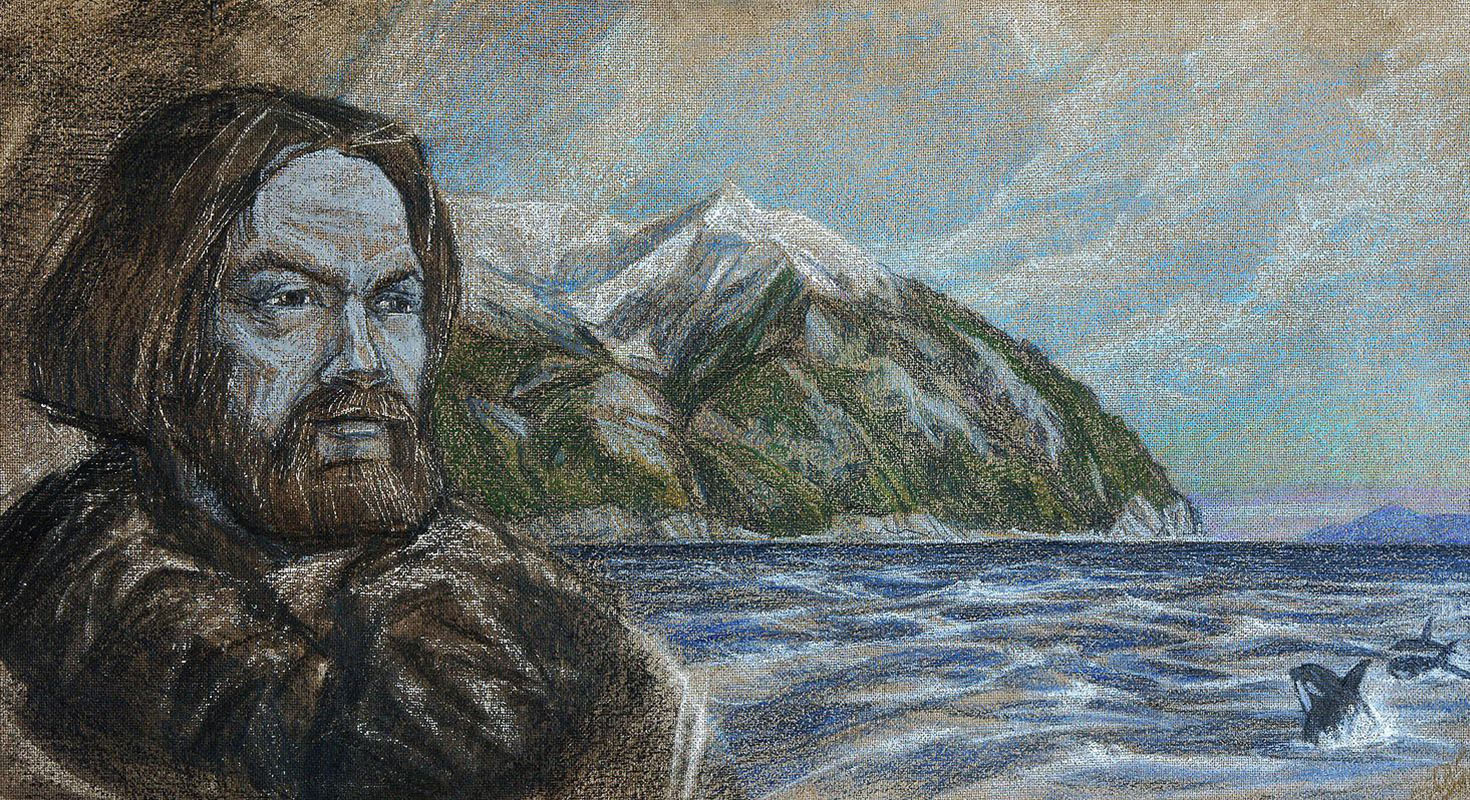
\includegraphics[scale=0.3]{Data/RYAV_predposylki/scRafIMHAjs.jpg}
	%	\label{fig:scipion} % Unique label used for referencing the figure in-text\end{document}
	%	%\addcontentsline{toc}{figure}{Figure \ref{fig:placeholder}} % Uncomment to add the figure to the table of contents%----------------------------------------------------------------------------------------
	\caption{Казак Иван Москвитин (современное изображение)}%	CHAPTER 2
\end{figure}

Но Дальний Восток оставался на картах Терра Инкогнитой еще долгие годы. Амур относился к Китаю, устье его не было изведано, а Сахалин – и вовсе считался полуостровом. Так продолжалось до губернаторства Н. Н. Муравьева. В середине XIX в. низовья Амура исследовали русские моряки. Экспедиция Геннадия Невельского основала Николаевский Пост.

В то время соперником Российской Империи была не Япония, а Китай. Русские политики добились выгодных условий с ослабленной опиумными войнами империей Цин. Айрапетов, автор монографии по истории Русско-японской войны так описывает это соглашение: 
\begin{textcitation}
\textit{«16(28) мая 1858 г. в гор. Айгун на правом берегу Амура ген. Н.Н. Муравьевым и князем И-Шанем был подписан русско-китайский договор. Левый берег Амура от реки Аргунь до берега моря переходил к России. Граница между государствами проводилась по Амуру вплоть до р. Уссури. Вопрос об Уссурийском крае оставался открытым, он объявлялся совместным владением Цинской и Российской империй. Реки Амур, Уссури и Сунгари открывались только для русского и китайского судоходства. Оба государства обязались оказывать покровительство общей торговле на обоих берегах Амура, маньчжурскому населению, жившему на левом берегу Амура, разрешалось остаться на жительство «под ведением маньчжурского правительства»}.
\end{textcitation}

\begin{figure}[h!tb] 
	\centering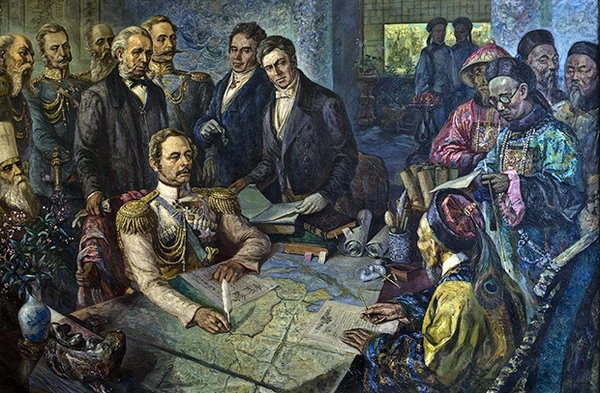
\includegraphics[scale=0.5]{Data/RYAV_predposylki/wvyqo2RYUXU.jpg}
	%	\label{fig:scipion} % Unique label used for referencing the figure in-text\end{document}
	%	%\addcontentsline{toc}{figure}{Figure \ref{fig:placeholder}} % Uncomment to add the figure to the table of contents%----------------------------------------------------------------------------------------
	\caption{Айгунский договор. Художник — В. С. Романов
	}%	CHAPTER 2
\end{figure}

Тремя годами ранее вице-адмирал Путятин и Тосиакирой Кавадзи подписали первый договор между Россией и Японией (Симодский трактат). Остров Сахалин объявили совместным владением двух империй, в дружбе заручились.

Освоение Приамурья шло медленно. Население состояло из забайкальских казаков, солдат и немногочисленных крестьян-переселенцев. Путь из центральной России вчерашних пахарей занимал два года. Два года они шли через океан лесов с рифами гор в суровом континентальном климате в полную неизвестность. На месте их ждало не Беловодье, а пустынные необитаемые болота, на обработку которых не хватало сил. Не лучше чувствовали себя и казаки, переброс которых на новую границу \textit{«сопровождался Библейским плачем»}.

С Китаем отношения оставались напряжёнными. В 70-е годы мы столкнулись с ним в Средней Азии. Тут же подоспел Лондон со своим страхом Russian Cossacks в Индии. На тот момент расклад был таков: Британия с Китаем против Российской Империи.

Китай стоило бояться даже ослабленный. Айрапетов пишет:
\begin{textcitation}
«Численность китайских войск (регулярной армии, маньчжурской конницы и запаса) в Маньчжурии к концу 80-х гг. XIX века доходила до 175 тыс. чел., в то время как на всем русском Дальнем Востоке им могли противостоять не более 23 800 чел». 
\end{textcitation}
Отряд из Центральной России в случае войны шел бы 18 месяцев.

Дальний Восток же являлся слабо заселенным отдаленным незащищенным рубежом. 11 тысяч русских, 3,5 тысячи корейцев, 3 тысячи китайцев, 4 тысячи местных народов – вот и все население Приморья в 1870-х гг.. 44 тысячи проживало в Приамурье.

Член комиссии Морского Министерства И. Чайковский в начале 80-х гг. так писал о Владивостоке:
\begin{textcitation} 
	«Число жителей, вместе с нижними чинами и их семействами, простирается до 8 800 душ, из которых инородцев, т. е. китайцев и корейцев, до 3 900 душ».
\end{textcitation}

В начале 1891 г. Александр III подписал указ о строительстве Транссиба, этого нового позвоночника Империи. Железная дорога требовалась еще и потому, что главный порт – Владивосток – на 4 месяца покрывался льдом. И корабли базировались у нашего союзника, Империи Восходящего Солнца, в Нагасаки.
Нагасаки посетил и наследник престола Николай II. Через несколько дней в Оцу безумный фанатик атаковал наследника престола. Распространено мнение, в частности, встречал я его в ролике Гоблина, в беседе с Борисом Юлиным, что, мол, тогда возникла первая трещина между Империями, а великий князь вел себя как дурак и чуть ли не мочился на храм. Это не так. Преступника покарали, инцидент старались всячески замять, вплоть до того, что синтоистские жрецы молились за здоровье будущего правителя, да и никаких источников о неподобающем поведения Николая Александровича не сохранилось, кроме слухов уровня кликбейтной рекламы.

\begin{figure}[h!tb] 
	\centering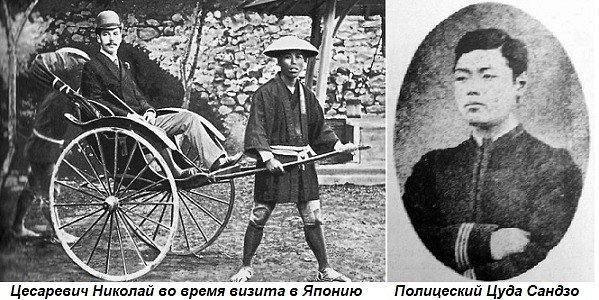
\includegraphics[scale=0.5]{Data/RYAV_predposylki/_d-EZ1r9Apk.jpg}
	%	\label{fig:scipion} % Unique label used for referencing the figure in-text\end{document}
	%	%\addcontentsline{toc}{figure}{Figure \ref{fig:placeholder}} % Uncomment to add the figure to the table of contents%----------------------------------------------------------------------------------------
	\caption{Айгунский договор. Художник — В. С. Романов
	}%	CHAPTER 2
\end{figure}

А через несколько недель Николай Александрович открыл Транссибирскую магистраль, что «превращала Россию в целостную континентальную структуру на огромном евразийском пространстве».
\begin{textcitation} 
«В начале 90-х гг. население Приморья и Приамурья насчитывало 182607 человек, из них 39722 горожан, 50916 крестьян, 26261 казаков, 14623 «инородца»(представители местных малых народов), 33000 китайцев, постоянно проживавших по праву, предоставленному им Айгунским договором 1858 года, 14684 корейца, 447 японцев, 117 «прочих иностранцев» и 2832 ссыльных. По сравнению с Маньчжурией, где проживало около 13 млн. человек, это были весьма слабо заселенные земли».
\end{textcitation}

\section{ Переворот в политике}

Японская империя стала соперником империи Российской лишь к концу XIX в. И не инцидент в Осу подтолкнул к соперничеству, а Корея. Экспансия являлась прямым продолжением революции Мэйдзи и модернизации экономики. Страна Восходящего Солнца зарилась на Страну Утренней Свежести с 1870-х гг.

Дорам, кей-попа и самсунга, равно как и атомного оружия, на корейском полуострове тогда еще не было. Ценностью считалась сама территория: Японцы объявили Корею «ножом, направленным в сердце».

Япония трижды, в 1875, 1882 и 1884 гг., планировала подчинить Корею, но не решалась из-за Китая. Лишь в 1894 г., во время крестьянского восстания, противостояние двух империй вылилось в войну.


\begin{figure}[h!tb] 
	\centering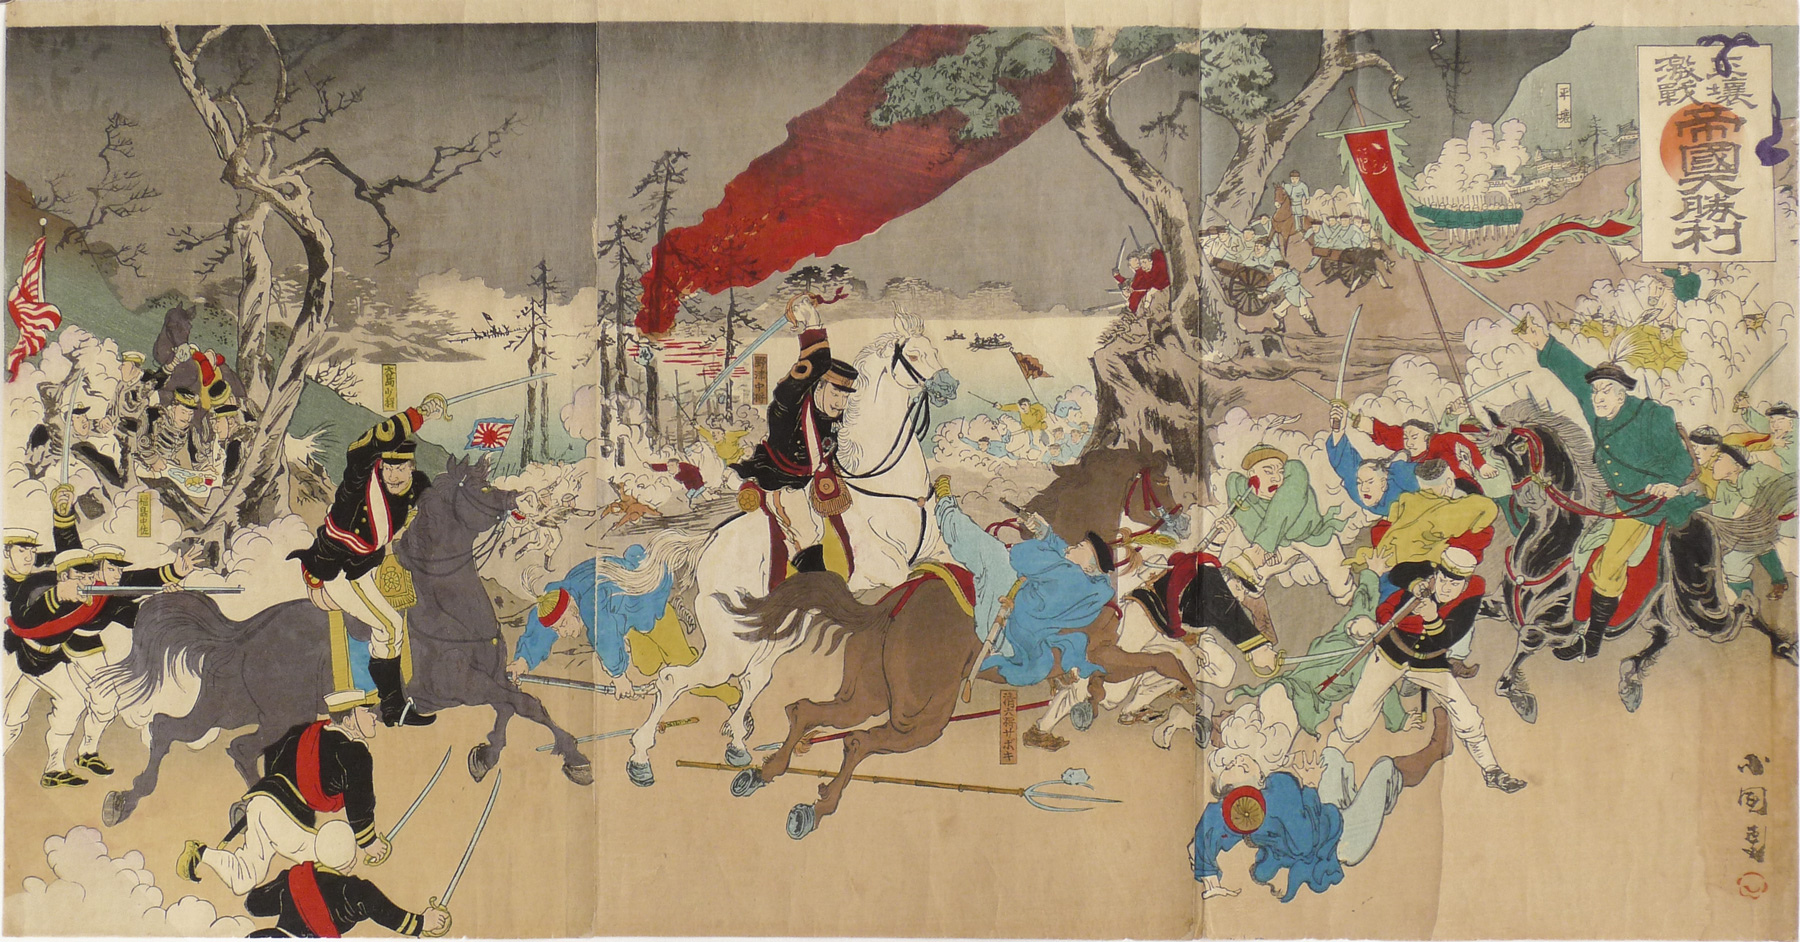
\includegraphics[scale=0.25]{Data/RYAV_predposylki/e2_wdd6jKoU.jpg}
	%	\label{fig:scipion} % Unique label used for referencing the figure in-text\end{document}
	%	%\addcontentsline{toc}{figure}{Figure \ref{fig:placeholder}} % Uncomment to add the figure to the table of contents%----------------------------------------------------------------------------------------
	\caption{Айгунский договор. Художник — В. С. Романов
	}%	CHAPTER 2
\end{figure}

Япония строила армию по образу германской. Модернизация дала плоды: во время битвы за Порт-Артур японцы потеряли по данным Айрапетова всего 400 чел., китайцы — около 4 тыс. Сражение у стен Пхеньяна также обернулось разгромом китайской армии. Цинская держава имела и броненосный флот, приобретенный на Западе. Но отсутствие навыков, как у моряков, так и у командиров, вкупе с коррупцией, привели к поражению и на море.

А пока в Корее гремела война, за тысячи километров, в Ливадийском дворце скончался царь-миротворец, Александр III. Власть получил Николай II.

Немало проблем беспокоило молодого императора. Но и Дальний Восток не оставался без внимания. Николай II, в отличие от своего отца, выступал за наращивание силы. В 1895 г. Морское министерство отправило телеграмму на берега Тихого Океана, приказав найти в Китае или Корее подходящий порт.

\begin{textcitation} 
30 марта (11 апреля) 1895 г. на Особом совещании министров под председательством Великого Князя Алексея Александровича было принято решение придерживаться политики дружбы со слабым соседом — Китаем. К этому времени стало ясно, что русское выступление в пользу status quo поддержат Франция и Германия
\end{textcitation}

Одним из самых активных ястребов стал Витте. А военные, в частности Начальник Главного штаба ген. Обручев, указывали на опасность противостояния в далеких краях, где в любой момент на помощь Японской империи могла прийти Империя Британская. Офицер сообщил и о недостатках инфраструктуры:

\begin{textcitation} 
По мнению начальника Главного штаба, для нас в высшей степени важно ни под каким видом не впутываться в войну. Необходимо иметь в виду, что нам пришлось бы воевать за десять тысяч верст с культурной страной, имеющей 40 миллионов населения и весьма развитую промышленность. Все предметы военного снаряжения Япония имеет у себя на месте, тогда как нам пришлось бы доставлять издалека каждое ружье, каждый патрон для наших войск
\end{textcitation}

Император принял точку зрения выступающего за статус-кво и ультиматума Японии Витте. В своем дневнике Николай II записал:
\begin{textcitation}  «Решили: настоять энергично на очищении японцами южной части Маньчжурии и Порт-Артура; если же они не послушаются совета, то принудить их к тому силой. Дай Бог, только не втянуться в войну!»
\end{textcitation}

В результате Россия вместе с Францией и Германией 23 апреля 1895 г. вмешались в японо-китайские переговоры и потребовали пересмотреть условия. «Тройственная интервенция» стала еще один шагом на пути к войне.

Япония отказалась от Ляодунского полуострова, где находился Порт-Артур. Россия приготовилась к экспансии.

\section{Разделение Китая}

В интернете часто можно встретить мнение, что вот, мол, японцы, были пешками клятых Британцев и не менее клятых США или что Коварная Англичанка столкнула лбами наивную Россию и ничего не понимающую Японию. Это не совсем так.
Россия, Британия, Япония, Германия и Франция делили Китай. Продвижение Российской Империи на прежних направлениях замедлилось. В Средней Азии шла «Большая Игра» с Британией. На Босфоре же Россию видеть не желал даже наш традиционный союзник – Германия. Кайзер Вильгельм II даже ездил в Османскую Империю, где провозгласил себя в Дамаске «другом всех мусульман». Дальний Восток, несмотря на соперников, казался наиболее перспективным – места много, не поссоримся.
В 1896 г. Россия и Китай подписали секретный союзный договор. Империя Цин давала созданному Русско-Китайским банком обществу КВЖД разрешение на строительство магистрали. Как пишет Рыбаченок И.С. в труде о внешней политике Российской державы на рубеже веков

\begin{textcitation}
	Выгоды были значительны: понижались китайские таможенные пошлины на товары, провозимые по КВЖД; устанавливались свои железнодорожные тарифы; доходы дороги освобождались от налогов и пошлин на пассажирский багаж и грузовой транзит; разрешалось беспошлинно ввозить каменный уголь для нужд дороги и на льготных условиях разрабатывать угольные копи в регионе. Вдоль линии содержалась собственная охранная стража. На чужой территории создавалось “как бы государство в государстве”
\end{textcitation}

\begin{figure}[h!tb] 
	\centering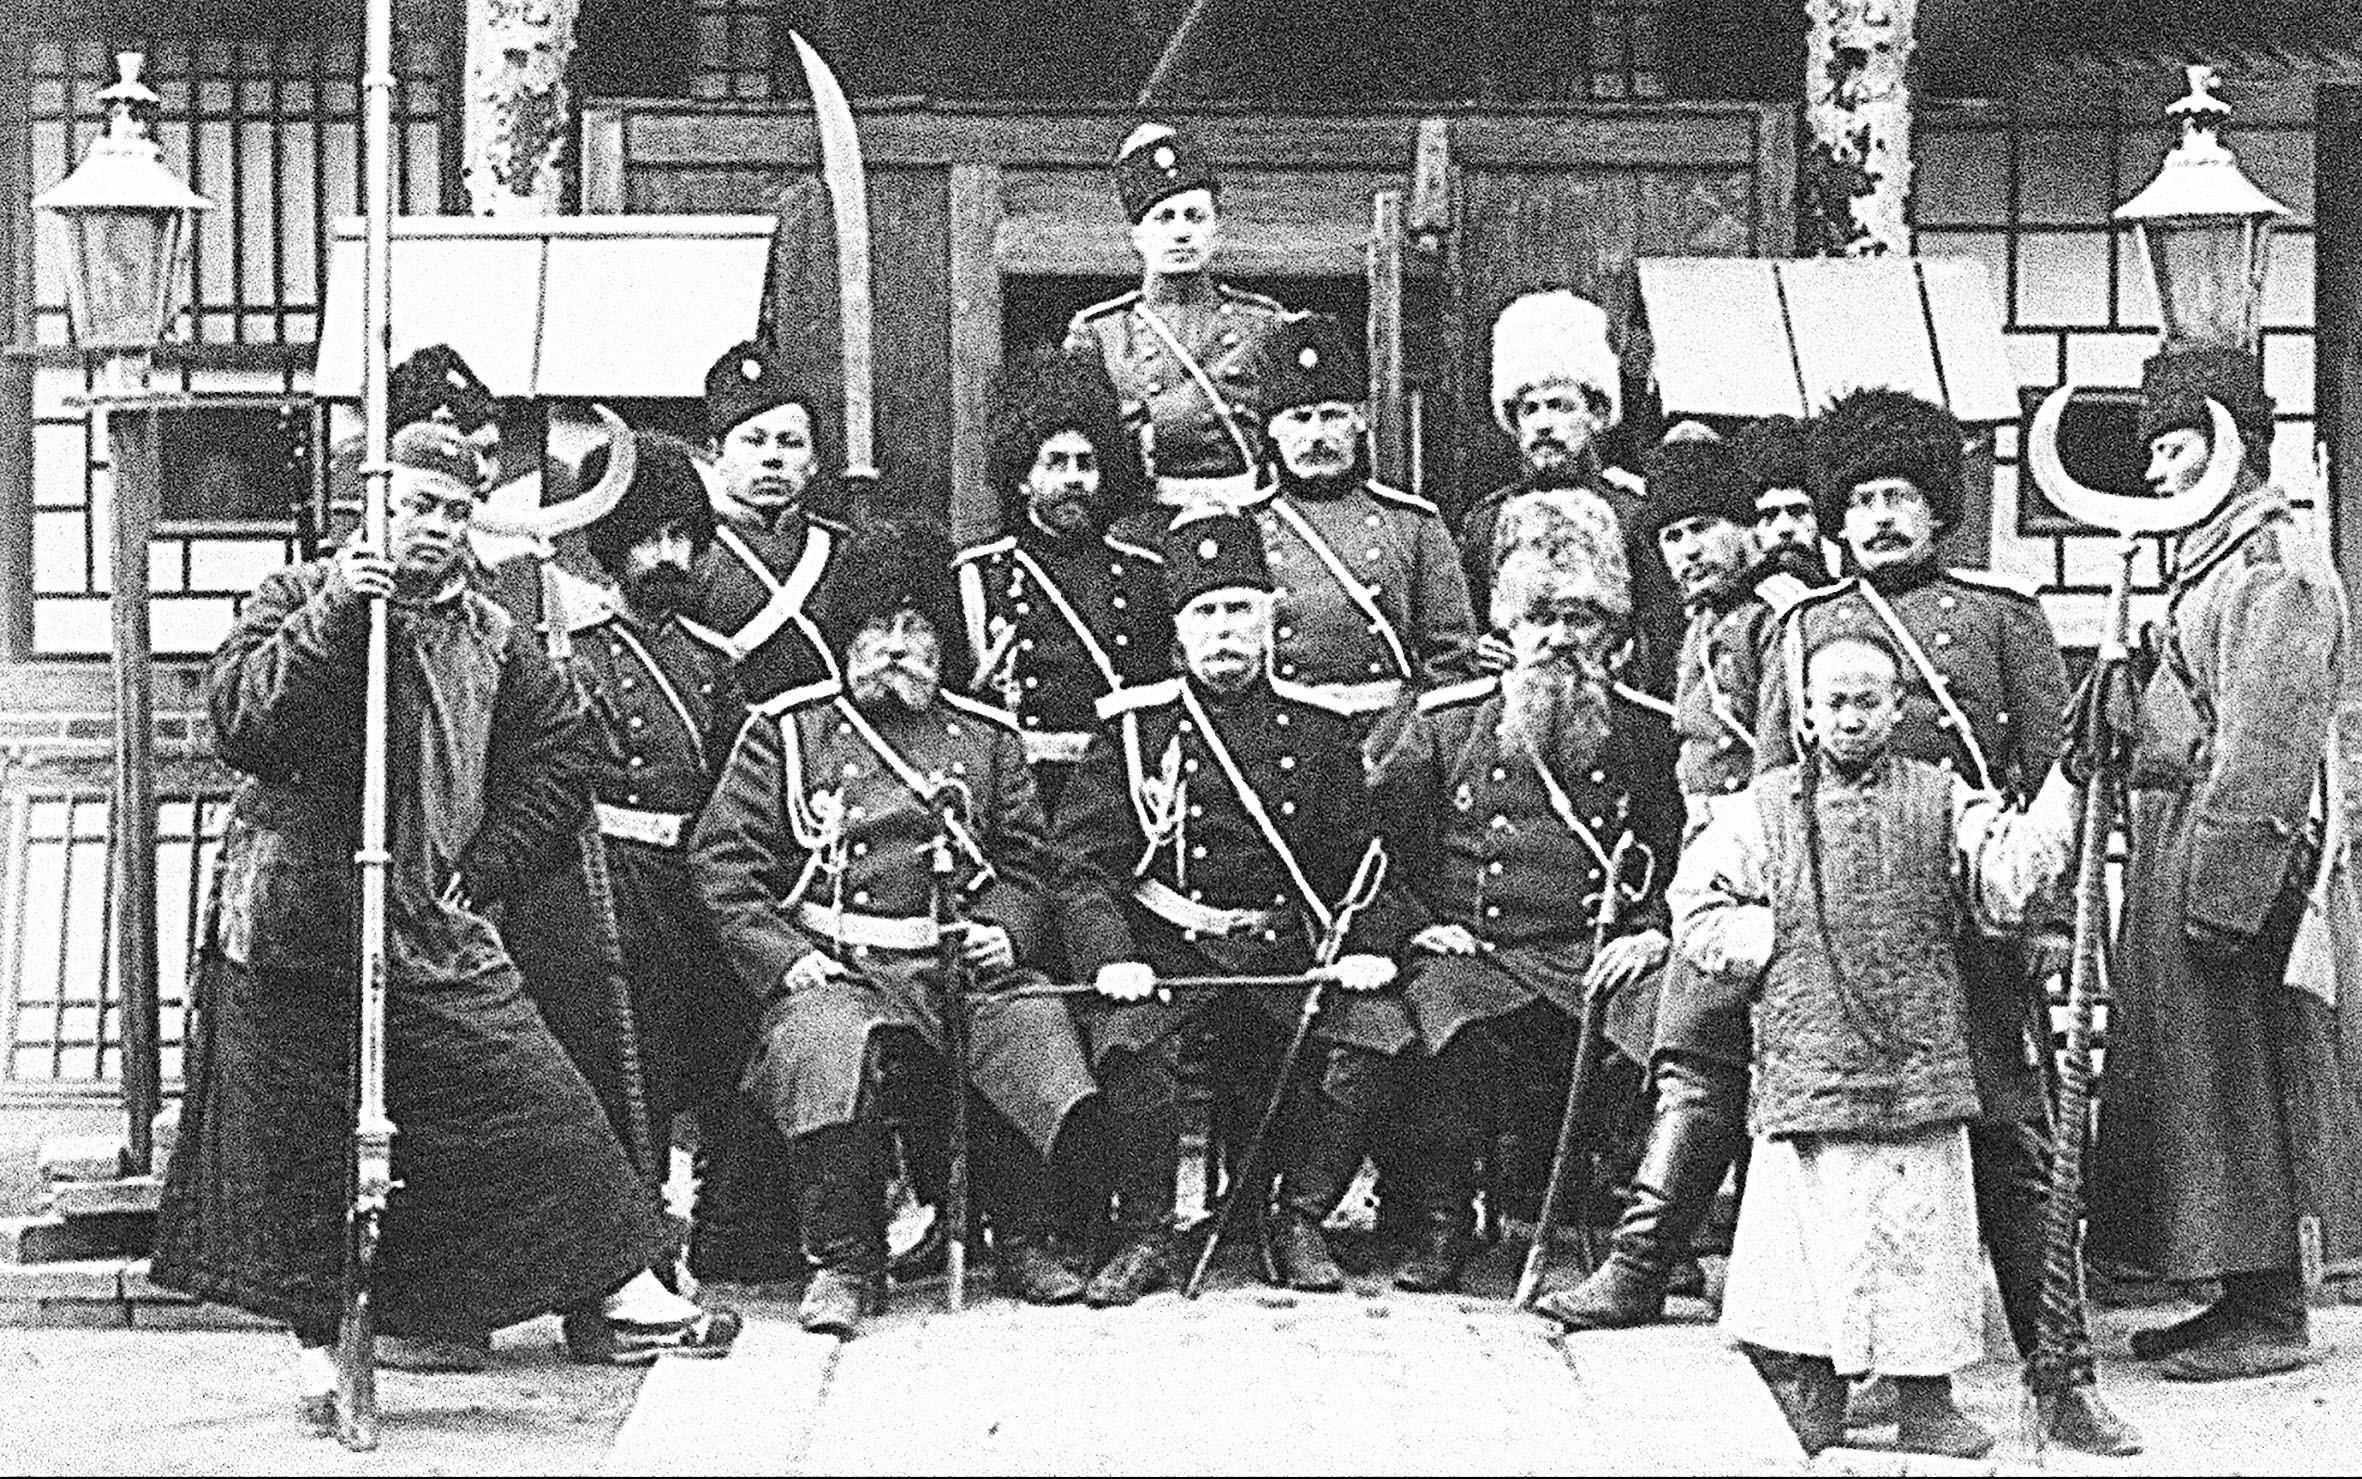
\includegraphics[scale=0.2]{Data/RYAV_predposylki/1snYqdEvc-k.jpg}
	%	\label{fig:scipion} % Unique label used for referencing the figure in-text\end{document}
	%	%\addcontentsline{toc}{figure}{Figure \ref{fig:placeholder}} % Uncomment to add the figure to the table of contents%----------------------------------------------------------------------------------------
	\caption{Пограничная стража КВЖД
	}%	CHAPTER 2
\end{figure}

КВЖД так и не стала прибыльным предприятием. Не удалось и заселить полосу вдоль железнодорожной колеи русским населением (Хотя в интернете я находил статьи о полумифической «Желтороссии»). Зато Российская Империя создала прецедент, которым воспользовались немцы, потребовавшие после убийства миссионеров порт Циндао от Китая.

Российская Империя не стала останавливать немцев. Николай II решил строить на Дальнем Востоке незамерзающий порт. Император заявил: \textit{«Я всегда был того мнения, что будущий наш открытый порт должен находиться или на Ляодунском полуострове, или в северо-восточном углу Корейского залива».} Китай не сразу согласился. 1 декабря 1897 г. наши корабли отправились на рейд Порт-Артура. Маневры обеспокоили не только китайское правительство, но и британцев. Русские суда у берегов Ляодуна встретил британский крейсер.

Столкновения между империями не случилось, хотя напряжение выросло. Но на стороне России оказалась Германия. Кайзер надеялся, что дальневосточные дела отвлекут Россию от европейских театров. И как только китайцы уступили немцам в Циндао, русские вошли в Порт-Артур. Десант из стрелкового полка и казачьей сотни высадился 17 (29) марта 1898 г. За день до этого Великий князь Кирилл Александрович поднял на вершине Золотой горы русский стяг.

Британия негодовала. Джозеф Чемберлен кричал в стенах парламента: «Если садишься обедать с чертом, ты должен взять с собой очень длинную ложку». В лицо англичане русских чертями не называли, но заявили, \textit{что занятие Россией военного порта поблизости от Пекина будет рассматриваться как начало раздела Китая}.

Великобритания даже думала заключить оборонительный союз с Германией, но общий антагонизм Лондона и Берлина помешал этому. Долгие дипломатические игры окончились разделением сфер влияния: «Россия обязывалась не препятствовать железнодорожным предприятиям Англии в районе Янцзы, а Англия – аналогичным предприятиям к северу от Китайской Стены». Также Британцы создали свою морскую базу в Вейхавее.

Японцев три базы трех различных государств тревожили не меньше, чем китайцев. Айрапетов приводит слава японского аристократа: \textit{Как зубы страдали бы от холода без губ, также и Японию ожидала бы трагическая судьба, если бы территория Китая была потеряна. А по движению западных держав на восток было ясно, что она скоро может быть потеряна}

Если Балканы являлись пороховой бочкой, то Дальний Восток целым военным складом. А самым опасным погребом в нем была Корея. В 1895 г. прояпонские придворные убили выступавшую за союз с Россией королеву Мин Менсон. Попытка русских офицеров создать из корейских солдат обученную армию провалилась. Инструкторы покинули страну.

Вскоре Российская Империя и Японская империя подписали договор о разграничении сфер влияния в Корее. Фактически полуостров перешел под контроль страны Восходящего Солнца.

\section{Восстание Боксеров.}

В конце XIX века и без того тяжкое положение Китая осложнилось из-за наводнений и засухи. Из одной провинции в другую шагал голод. В казне не хватало денег на солдат, и все больше воинов уходило, куда глаза глядят.
Одновременно Китай изматывали иностранцы. Железные дороги уничтожали поля, а новые технологии оставляли без работы ремесленников. Не любили китайцы и миссионеров, хотя немало жителей Поднебесной откликнулись на проповеди: количество христиан исчислялось сотнями тысяч.
Ненависть к лаоваям стала выливаться в волнения. Их организовывали тайные общества. Они решили выгнать иностранцев из страны.
Про восстание Ихэтуаней написано немало. А вот так их видели русские люди в Китае:

\begin{textcitation}
Двор кумирни «Хо Шэнь Мяо», посвященной «Духу огня» и расположенной в глубине китайского города Тяньцзина, был переполнен ихэтуанцами.
У всех в руках были зажженные красные бумажные фонари на палках. Головы были обмотаны красными платками, под которыми были свернуты косы. На голой груди висел красный платок с написанным таинственным иероглифом. Красный пояс, свернутый узлом с заткнутым большим кривым ножом, туго сжимал худощавое, смуглое тело. На ногах были широкие синие шаровары, перехваченные у ступни красными перевязками
\end{textcitation}

\begin{textcitation}
Их магические методы состоят из множества заклинаний, содержащих в себе по 8-12 или 16–20 иероглифов, которые составляют 10 фраз. Они (т. е. наставники ихэтуаней, среди которых было много детей и подростков. — Н.А., С.Л.) заставляют подростков читать их наизусть, держа глаза закрытыми и кланяясь по три раза подряд на Юг. [Потом] те ложатся рядами на землю и через короткий промежуток времени вскакивают, выкрикивая свое имя и фамилию, которые оказываются именами героев древних династий. Подростки начинают делать бойцовские движения, то приближаясь друг к другу, то удаляясь. Некоторые из них держат в руках бамбуковые палки определенной длины, похожие на пики, алебарды, обоюдоострые мечи и сабли. Рассеявшись по горным проходам и ущельям, они буйствуют, переворачивая все вверх дном…
\end{textcitation}
\begin{textcitation}
Чжань, один из главных предводителей боксеров, быстро прошел вперед и стал на ступенях кумирни. Он был одет во все красное: красная чалма на голове, красная шелковая кофта, красные шаровары, пояс и подвязки и надетые поверх шаровар красные набедренники с нашитыми иероглифами Цзи — Счастье. На груди был вышит неведомый знак, под которым скрывалась чудесная ладанка с зашитыми в ней 3 корешками имбиря, 21 зерном черного гороха и 21 зерном красного перца. В руках у него было длинное копье с красной кистью под острием. За поясом нож и две кривые сабли в одних ножнах, а за плечами колчан с луком и стрелами.
Четыреста дней Чжань упражнялся в науке и колдовствах ихэтуанцев, четыреста дней Чжань искушался в посте и молитвах и из «мутного» Хунь он сделался «светлым» Цин. Он стал недоступен наваждению злых духов, болезням, несчастиям, голоду и смерти. Ему не страшно заморское огнестрельное оружие, в котором он не нуждается, так как верит только в силу своей родной сабли, ножа и китайского копья.
Он верит в справедливость и безпредельное всемогущество Неба — Тен и великого небожителя, бога войны Гуань-лао-е, которые [99] всегда спасали Срединный народ от злых подземных духов, а теперь спасут от земных белых дьяволов.
\end{textcitation}

В мае 1900 г. боксеры взяли Пекин. В этот же месяц в Порт-Артуре русские офицеры провели первый бал. Военные не удивились известиям об очередном восстании.

\begin{figure}[h!tb] 
	\centering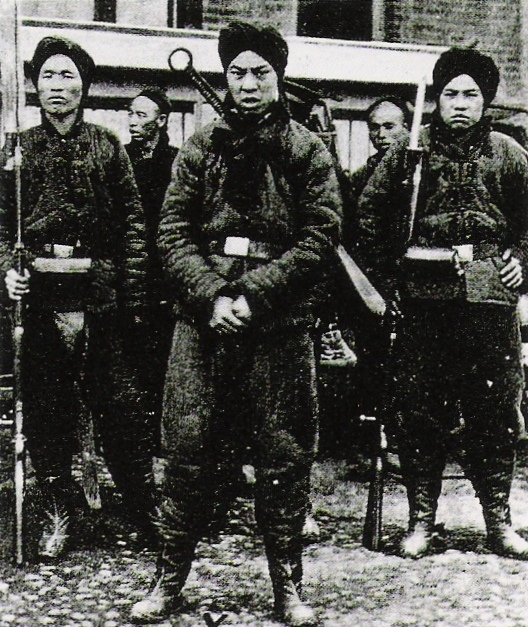
\includegraphics[scale=0.5]{Data/RYAV_predposylki/hk4dFO3QF1g.jpg}
	%	\label{fig:scipion} % Unique label used for referencing the figure in-text\end{document}
	%	%\addcontentsline{toc}{figure}{Figure \ref{fig:placeholder}} % Uncomment to add the figure to the table of contents%----------------------------------------------------------------------------------------
	\caption{Боксеры
	}%	CHAPTER 2
\end{figure}

Но уже в июне началась осада посольского квартала, где находились и русские дипломаты. Незадолго до этого в Пекин пытался прорваться созданный из солдат различных держав отряд британский офицер Э. Сеймур. Русские воины так же вошли в него. Вице-адмирал Алексеев обратился к ним со словами:

\begin{textcitation}
	«Будьте тверды, выносливы, строго соблюдайте дисциплину, не обижайте мирных жителей. Помните, что русский солдат прежде всего христианин, а потому должен быть добрым к тем, кто не делает ему вреда. Ваши предки не раз доказали это».
\end{textcitation}

\begin{figure}[h!tb] 
	\centering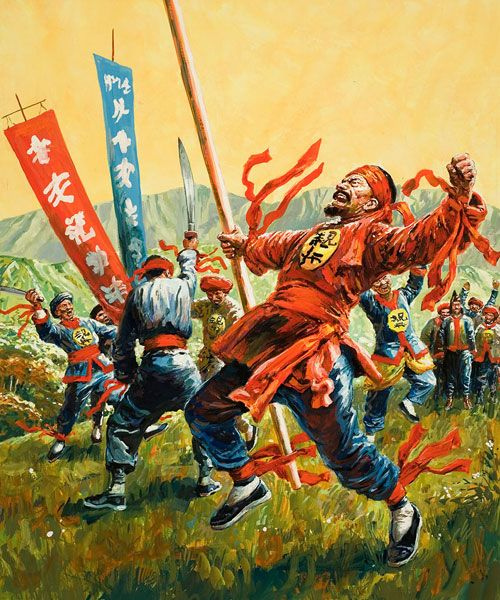
\includegraphics[scale=0.5]{Data/RYAV_predposylki/uWfCsUtq3gw.jpg}
	%	\label{fig:scipion} % Unique label used for referencing the figure in-text\end{document}
	%	%\addcontentsline{toc}{figure}{Figure \ref{fig:placeholder}} % Uncomment to add the figure to the table of contents%----------------------------------------------------------------------------------------
	\caption{Современный рисунок, изображающий боксеров
	}%	CHAPTER 2
\end{figure}

Но поход Сеймура провалился. Боксеры оказались сильней. Русский полк потерял 15\% своего состава.
21 июня восставших поддержало правительство по приказу императрицы Цы Си. Ее имя известно не только знатокам истории Востока. Драгоценная наложница, пережившая и «официальную императрицу», и своего сына, и остановившая не из-за консерватизма, но из-за боязни потерять власть сто дней реформ, отчаянно металась между ихэтуанями и иностранцами и перешла, в конце концов, на сторону повстанцев.

Восстание Ихэтуаней отразилось и на обстановке в Маньчжурии. Все чаще на КВЖД нападали хунхузы – разбойники северного Китая. К началу 20-ого века они, пользуясь слабостью власти на китайском фронтире, превратились в организованные преступные синдикаты. К ним присоединились боксеры, а потом и армия.

К 1898 г. охрана КВЖД насчитывала 5000 человек. Но даже их не хватало, чтоб контролировать тонкую ниточку железнодорожного тракта. Русское население сконцентрировалось в Харбине. Женщин и детей отослали в Хабаровск.

24 июня появилось Высочайшее повеление о формировании 51 Восточно-Сибирской стрелковой бригады. 26 июня – Высочайшее повеление о вступлении в Маньчжурию. Но уже в начале июля китайцы принялись бомбардировать Благовещенск, и атаковать корабли по Амуру.

Войск не хватало. «Численность Амурского казачьего войска, размещенного по левому берегу этой реки от станицы Покровской до выселка Забеловского — всего на 1800 верст. На 1 января 1899 г. проживало 24 562 человека, из них казаков — 11 363(всех возрастов) и 10 568 казачек».

К осени на Дальний Восток по железной дороге и по морю перебросили около сотни тысяч солдат. Несмотря на проблемы с инфраструктурой, Маньчжурию русские взяли. И хотя русским пришлось воевать с партизанскими отрядами «Армии чести и справедливости», победа осталась за Российской Империей.
Правительство российской Империи стремилось действовать в районе КВЖД. Но ввод войск в Маньчжурию вызвал беспокойство у Японцев. Империя Восходящего Солнца стала искать сближения с Великобританией.


\section{Навстречу к войне
}

В начале XX века на корабль под названием Россия, точнее на его курс во внешней политике, действовало несколько сил. Военные понимали каким штормом обернется для нас война. Витте предлагал умеренное продвижение. Наконец, часть придворных, вошедшая в историю как «безобразовская клика», во главе с А. Безобразовым и генерал-адъютантом Алексеевым двигала судно прямым курсом, словно не зная о рифах и водоворотах.
Сейчас ряд ученых пришли к выводу о незначительном различии между «Безобразовцами» и Витте. Все сводилась лишь в темпе, а цели были одинаковыми.
Витте видел Запад источником капиталов, а Восток рынком для сбыта русских товаров. Связующим звеном между частями Света, которым никогда не сойтись, служила Россия и ее Транссибирская магистраль. Государственный деятель хотел провести ветку от Дальнего Востока к Корейским портам и включить Страну Утренней Свежести в свою зону влияния. Для достижения целей был создан Русско-Корейский банк.
«Безобразовцы» же шли напролом. Еще в 1898 г. Николай II велел выделить деньги для концессии на реке Ялу. Даже министр Куропаткин не был в курсе о текущих делами.

\begin{figure}[h!tb] 
	\centering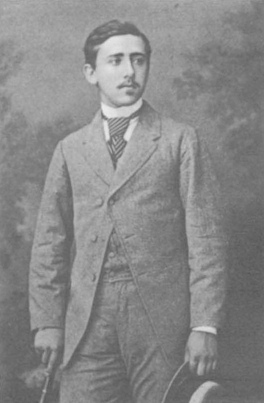
\includegraphics[scale=0.6]{Data/RYAV_predposylki/Y7AQ96Nf2A4.jpg}
	%	\label{fig:scipion} % Unique label used for referencing the figure in-text\end{document}
	%	%\addcontentsline{toc}{figure}{Figure \ref{fig:placeholder}} % Uncomment to add the figure to the table of contents%----------------------------------------------------------------------------------------
	\caption{А. Безобразов		
	}%	CHAPTER 2
\end{figure}

Концессия стала прикрытием для проникновения в Корею. Денег она не принесла: «Безобразов, обещавший в 1903 г. доход от концессии на Ялу в 5 млн. рублей, и в 1904 г. в 10 млн. рублей, смог к концу 1903 г. обеспечить лесом только один пароход, а так как их было зафрахтовано два, то на второй пришлось покупать лес в Америке».
Генерал Алексеев возглавил наместничество, созданного из Квантунской области и приамурского генерал-губернаторства. Император писал: «Мой Наместник на Дальнем Востоке есть естественный Главнокомандующий всеми сухопутными и морскими силами края, призванными высоко держать русское знамя и служить надежной охраной наших справедливых интересов на берегах Тихого океана». Сам генерал мечтал же о присоединении Маньчжурии.
Военный министр Куропаткин в том же году посетил Японию и Дальний Восток. Вернулся он с двойственными впечатлениями. Он опасался сил японцев, но считал, что русская армия на далеких границах даст им отпор.
Разобщенность приводила к неразберихе, а она, в свою очередь, к войне и поражению.
В 1903 г. истек и срок вывода войск из Маньчжурии. Но армия так и осталась в Китае, оправдывая свое нахождение невыполнением уже обязанностей китайской стороны.
Японцы пытались найти язык с Российской Империей. Но их требования отвергала даже умеренная партия, состоявшая из Витте и министра иностранных дел Ламсдорфа. Безобразовцы же выждали максимально жесткую позицию. Уступать не хотел никто.
Параллельно японцы разрабатывали план военных действий и приступили к разведке в Корее и Маньчжурии. Начались учебные сборы. Активность их не скрывалось под пеленой тумана. Российская разведка вела наблюдения:

\begin{textcitation}
	Армия работает от солдата до фельдмаршала; работает может быть слишком лихорадочно, спешно, а потому и не всегда целесообразно, но упорно и настойчиво. До сих пор, все, что заимствовали японцы в области искусства у своих соседей, они сумели представить в новом, слегка измененном, но усовершенствованном виде… Способны ли японцы поставить на такую же высоту военное искусство — скажет решительное и авторитетное слово беспристрастное будущее
\end{textcitation}

Но знал ли об этом император? Как-то раз Ламсдорф передал Николаю II тезисы Куропаткина о японской армии и получил ответ: «это все-таки не настоящее войско, и если бы нам пришлось иметь с ним дело, то простите за выражение, но от них лишь мокро останется»


Надо отдельно сказать несколько слов о других державах. Какой-то объединённой коалиции, как в Крымскую Войну, против России не существовало. Каждый преследовал свои интересы. Великобритания надеялась, что столкновение России на Дальнем Востоке отвлечет Николая II от «Большой Игры». Еще в 1902 г. Лондон заключил с Токио союз. Он косвенно нейтрализовал и Францию. Берлин же рассчитывал, что прокси-конфликт Петербурга и Лондона выльется в открытое европейское соперничество и вернет былые дружеские отношения Российской империи и Германии. Наконец, Япония смогла заручиться поддержкой США и Китая. Россия оказалась в одиночестве.

Но у Российской империи остался еще один союзник, сильный и страшный – Время. Модернизация инфраструктуры, составление планов, усиление флота и работа дипломатов в конце концов дали перевес бы именно русским. Империя Восходящего Солнца стояла перед узким проливом и малейшее промедление грозило бы крахом.

И они решились.

В январе 1904 г. еще шли переговоры. 22 января в Токио отправилась очередная телеграмма. Но японцы по совету англичан задержали ее.

А 23 января японцы начали десантную операцию в Корее. 24 января – захватили русский пароход. 27 атаковали стоящие на рейде Русские корабли.

Война началась.

Источники:
\begin{itemize}
	\item Лукоянов И.В. «Не отстать от держав…» Россия на Дальнем Востоке в конце XIX – начале XX вв. – СПб.: Нестор-История, 2008. — 668 с.
	\item Айрапетов О.Р. На пути к краху. Русско-японская война 1904-1905 гг. Военно-политическая история. М.: Торговый дом "Алгоритм", 2014- 496 с.
	\item Рыбаченок И.С. Закат великой державы. Внешняя политика России на рубеже XIX-XX вв.: цели, задачи и методы. М.: РОССПЭН, 2012 - 582 с.
\end{itemize}


Автор Виктор Пепелов. Оригинал \url{https://vk.com/wall-162479647_108741}

\#Пепел@catx2

\#Заметка@catx2
